\subsection{Triển khai mô hình bằng Streamlit}
Trong đoạn mã, trước tiên chúng ta cần import các thư viện cần thiết như Streamlit, torch, joblib, cv2, numpy và các module khác.

Sau đó, chúng ta có hai hàm chính: faster\_rcnn\_detection và hog\_svm\_detection.

Trong hàm faster\_rcnn\_detection, ta mở ảnh đầu vào và khởi tạo mô hình Faster R-CNN pre-trained. Mô hình này đã được tinh chỉnh để nhận dạng người đi bộ. Sau đó, ta tải trọng số đã được huấn luyện từ tệp model\_30.pt. Tiếp theo, ta sử dụng mô hình để dự đoán trên ảnh và lấy ra các hộp giới hạn (bounding boxes) được dự đoán, nhãn tương ứng và độ tin cậy (score) của các nhãn. Chúng ta sử dụng ngưỡng (threshold) 0.8 để lọc các dự đoán có độ tin cậy cao. Cuối cùng, chúng ta vẽ các hộp giới hạn và thông tin nhãn lên ảnh và hiển thị ảnh kết quả.

Trong hàm hog\_svm\_detection, ta tải mô hình SVM đã được huấn luyện từ tệp models.dat. Tiếp theo, chúng ta tiến hành xử lý ảnh đầu vào bằng phương pháp HOG (Histogram of Oriented Gradients) và duyệt qua các cửa sổ trượt (sliding windows) trên ảnh. Với mỗi cửa sổ, ta rút trích đặc trưng HOG và sử dụng mô hình SVM để dự đoán xem cửa sổ đó có chứa người đi bộ hay không. Nếu dự đoán là positive, ta lưu lại thông tin về vị trí và độ tin cậy của cửa sổ. Tiếp theo, chúng ta sử dụng non-maximum suppression để loại bỏ các hộp giới hạn trùng lắp và chỉ giữ lại hộp giới hạn có độ tin cậy cao nhất. Cuối cùng, chúng ta vẽ các hộp giới hạn đã lựa chọn lên ảnh và hiển thị ảnh kết quả.

Cuối cùng, trong hàm main, chúng ta sử dụng Streamlit để tạo giao diện người dùng. Người dùng có thể tải lên một tệp ảnh và xem kết quả phát hiện người đi bộ sử dụng cả hai phương pháp Faster R-CNN và HOG+SVM. Kết quả sẽ được hiển thị trên trang web Streamlit.

Qua đó, việc triển khai mô hình trên Streamlit cho phép người dùng tải lên ảnh và trực quan hóa kết quả phát hiện người đi bộ sử dụng hai phương pháp khác nhau, giúp phân tích và so sánh hiệu suất của các phương pháp trong bài toán này.

\begin{figure}[h!]
  \centering
  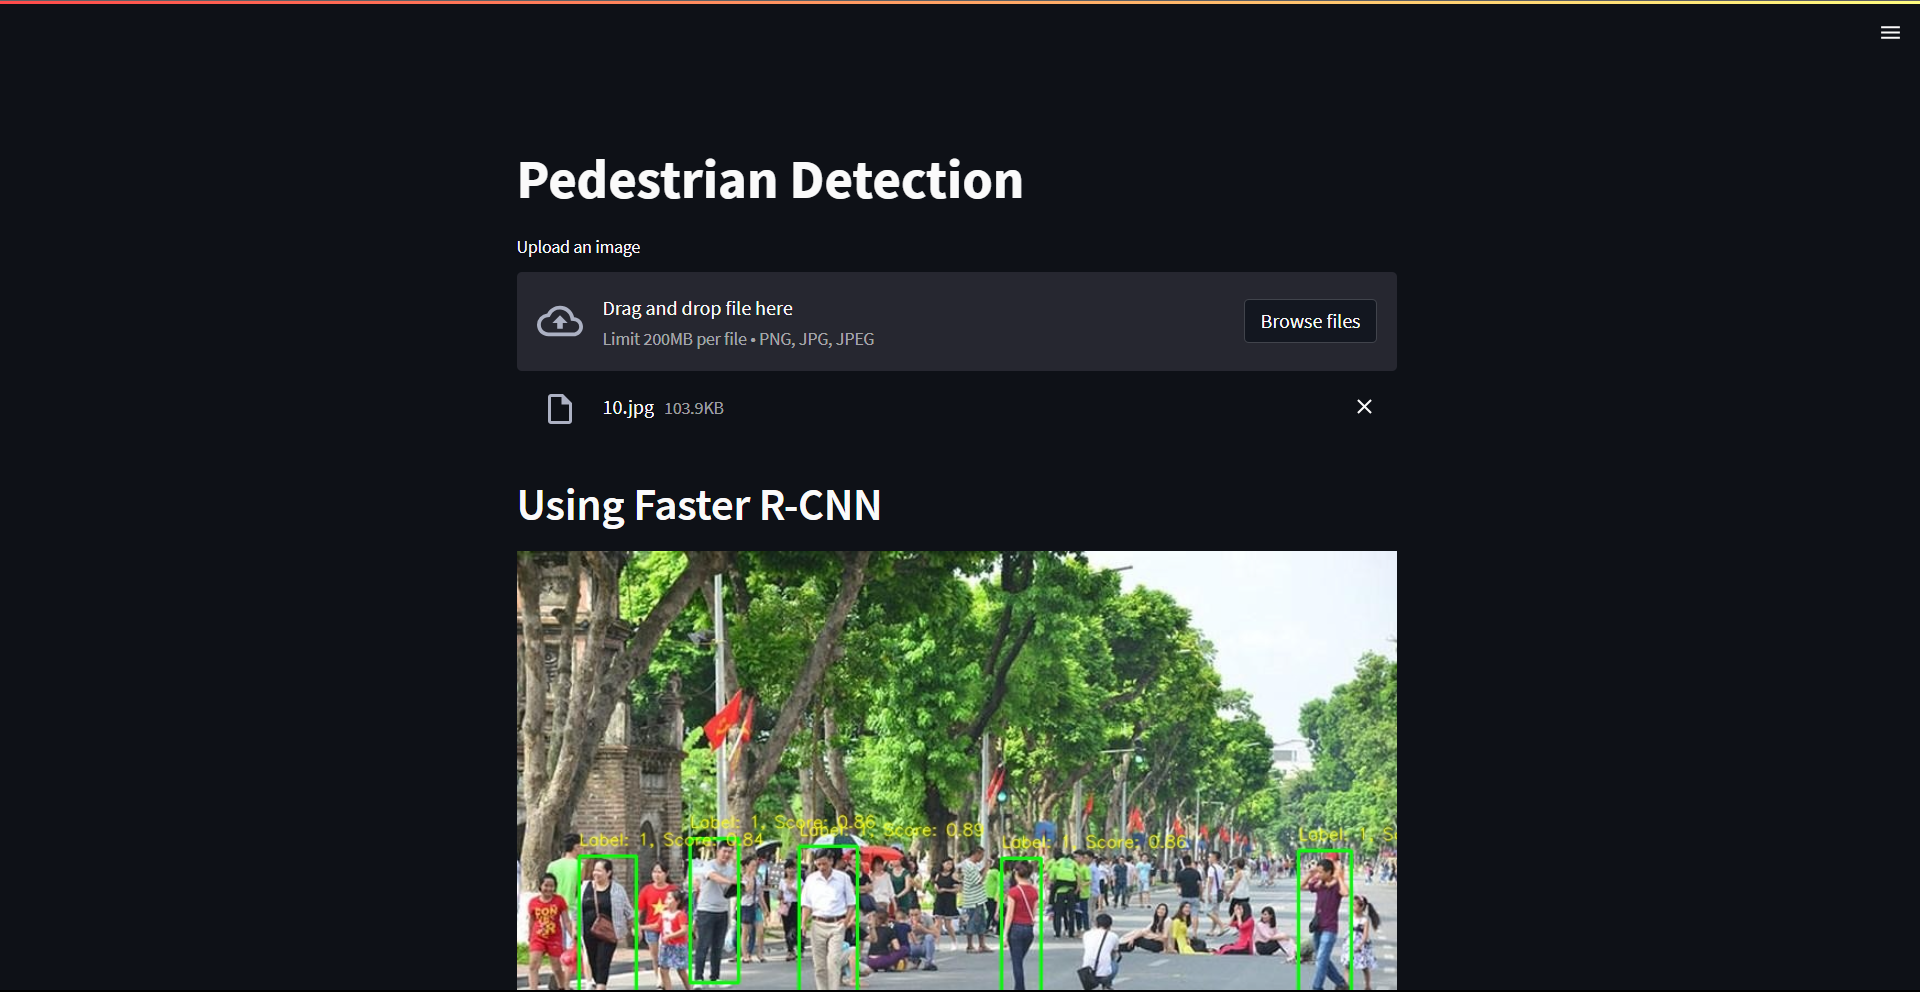
\includegraphics[scale=0.35]{graphics/streamlit.png}
  \caption{Deploy mô hình trên local host website bằng Streamlit}
\end{figure}